\chapter{Literature Survey} \label{lit}

Systematic reviews have many different stages that propose themselves as a candidate for automation. This section is going to look at the techniques that have been applied for some of these stages in previous literature.


\section{Steps of a Systematic Review} \label{stepssr}

It is useful for us to break down the steps involved in creating a systematic review into subtasks. This way we can observe what techniques can be applied during the relevant sub tasks to improve the efficiency of the process. The following definitions are derived task simplifactions from the cochrane tutorial on systematic reviews: \cite{cochranes}.

\begin{enumerate}
  \item Question definition.
  \item Relevant literature search.
  \item Data Filtering.
  \item Data Extraction.
  \item Analysis and Data combination.
\end{enumerate}

\subsection{Question Definition}

One of the best known techniques for formulating a systematic review question is known as the PICO strategy \cite{pico}. This technique focuses on exposing 4 pieces of information in the systematic review question: patient population, intervention or exposure, comparison or control and outcome.

Example: (credit goes to \cite{pico})

"Is animal-assisted therapy more effective than music therapy in managing aggressive behaviour in elderly people with dementia?"

\begin{center}
\begin{tabular}{ |c|c| } 
 \hline
 P & elderly patients with dementia \\ 
 I & animal-assisted therapy \\ 
 C & music therapy \\ 
 O & aggressive behaviour \\ 
 \hline
\end{tabular}
\end{center}

A potential point of interest would be attempting to generate these questions automatically given some literature context.

\subsection{Relevant Literature Search}

After formulating a question, systematic reviews need to search for the relevant literature that surrounds this question.

Large medical database-such as Pubmed \footnote{https://www.ncbi.nlm.nih.gov/pubmed/} contain relevant studies that can be selected for inclusion in a review. These databases are typically very large and require queries to retrieve data. These queries are structured, but not considered precise, as there is a strong emphasis on maximizing recall at the expense of precision. 

Naturally this can be modelled as an information retrieval problem. We have a large number of documents and we wish to retrieve all of the relevant ones. Reviewers will aim to retrieve all of the relavent studies, this is because there is a emphasis achieving a binary result set of relevant studies, as opposed to rankings studies by relevance.  

An important aspect of the relevant literature search step is the construction of the query. Query creators often apply filters (also known as hedges) \footnote{\url{https://hiru.mcmaster.ca/hiru/HIRU_Hedges_home.aspx}} to increase the effectiveness or/and the efficiency of the searching. Two key attributes for the query are the precision and the recall. By including synonymous phrases e.g: quality adjusted life or quality of well-being or disability adjusted life the recall can be increased, but at expense of the precision. The creation of this query is a task that could potentially have some aspects of NLP applied to it.


\subsection{Data Filtering}

The data filter stage involves reducing the amount of documents returned by the initial query down to a smaller subset of relevant document. This is done by idenfiying which retrieved studies match the inclusion criteria as defined by the PICO question.  This is can also be referred to as the abstract screening phrase \cite{Kanoulas12017}.

The length of this stage is highly dependent on how many documents were returned by the initial query, often in the excess of 5000 studies for a single query. In response to this, stopping criteria methods have been proposed that aim to optimize two key parameters; the effort and the recall. That is to say we want to get as many relevant documents as possible, whilst looking at the fewest. Examples of approaches include the knee method \cite{Satopa11} and the target method \cite{Cormack2016}. Other techniques could be applied and evaluated such as curve fitting, which is later examined in \ref{stops}

\subsection{Data Extraction}

The data extraction phase involves pulling the relevant information from the filtered subset of studies. Examples of important information includes how many people took part in the study and what the results were.

Being able to extract the relevant information from studies presents itself as an information extraction problem. The task to automate the process of extracting relevant information would reduce time and complexities of manually reviewing studies \cite{Siddhartha2015}.



\iffalse
\section{Indexing and Querying Medline and Automated Query Generation} \label{medlinelit}

Medline is a bibliographic database of published medical literature. Typically each entity will contain a title and an abstract containing some information on the study. Whilest Medline as a whole is very easy to access \cite{medline}, the large size and complexity of the data makes it difficult to retrieve the relevant information.

\subsection{Automated Query Generation} \label{aqglit}

Being able to automate query generation for literature searching would save systematic reviewers a significant amount of time. However, medical literature queries are typically complex and contain multiple levels of logical operators and synonymous term look ups. This makes the task of creating a query manually is a challenging task.



\subsubsection{Rapid Automatic Keyword Extraction Algorithm} \label{rakelit}

Rapid automatic keyword extraction (RAKE) is a keyword extraction algorithm \cite{rake}. This algorithm is used for taking the key pieces of information from text and is useful the domain of information extraction. This algorithm is of interest as it has potential usage within the field of query generation.

RAKE heavily relies on stop-words and punctuation separators as an indicator for the importance of a phrases and words. RAKE will iterate over sequences of words until a stop-word or separator is found, this phrase/word is then split and extracted. Frequency of occurrence (tf) and word co-occurrence matrices can then be used to reduce the key-word set down further.

RAKE can be further optimized by specifying minimum term frequency rates to capture more prominent terms.

\fi

\section{Stopping Criteria} \label{stops}

Stopping criteria is about finding the optimum point to stop reviewing a set of documents. This is important in a decision making process for maximizing efficiency. Consider having 100 relevant documents, where each document contains a binary indicator of being relevant or non-relevant. If we looked at 1/3 of these documents and saw a trend of positive values, we could use this to infer the reliability of the remaining documents.

Two key methods have been proposed for finding stopping points so far, the target method \cite{Satopa11} and the knee method. \cite{Cormack2016}. Both these methods are discussed below \ref{methods}



\subsection{Evaluation Metrics for Finding Stopping Points} \label{evalsstops}

In order to evaluate the suitability of stopping methods, we will use two evaluation metrics. The recall, which is the number of documents returned for a topic, and effort which is the number of documents that had to be examined. The challenge of finding a stopping point is optimizing both of these parameters. We could look at everything in our rankings to obtain a perfect recall score, but at the consequence of making 100\% effort.

\begin{equation}
Recall = \frac{|R|}{|D|}
\end{equation}

Where $R$ is the set of relevant documents found and $D$ is the set of all relevant documents.

Similarly, effort is computed as:

\begin{equation}
Effort = \frac{|L|}{|D|}
\end{equation}

Where $L$ is the set of documents that were examined.

Naturally we could exclusively optimized each of the parameters by either returning everything in the document collection ($R$ = $|D|$) or by just looking at a single document. ($L$ = 1)

Therefore it becomes difficult for us to evaluate our stopping criteria as we need to consider both of these parameters adjacently.

In response to this we can make use of two more evaluation metrics that were proposed by Cormack and Grossman \cite{Cormack2016}:

\begin{equation}
reliability = P [acceptable(S) == 1]
\end{equation}

reliability is computed over all searches and is read as the probability of the acceptability being 1. Where acceptability is calculated as:

\begin{equation}
  acceptability(S)=\begin{cases}
    1, & \text{$recall(S)>=0.7$}.\\
    0, & \text{$recall(S)<0.7$}.
  \end{cases}
\end{equation}

A stopping point is deemed to be acceptabl*e if 70\% of the relevant documents have been found \cite{Cormack2016}. As such, the reliability is an average over a search method. In Cormack and Grossman \cite{Cormack2016} a target is set of achieving 95\% reliability. Setting a acceptability score above 70\% will increase the amount of effort needed to reach the reliability threshold. In practise 70\% recall is not considered a sufficient amount of documents to retrieve, but as existing work in this area uses this figure, it is easier for us to compare results.


\subsection{Formulating Stopping Problem} \label{stoppingProblem}

In some cases, reviewers might be content in missing a proportion of relevant documents if a certain level of recall could still be guaranteed. This problem can be defined as a multi-objective optimization problem. We want to simultaneously optimize two competing objectives: maximization of recall recall and minimization of effort. 

We can use linear scalarization \cite{Noghin2015} as a simple way of optimizing both of these objectives. We define our problem as follows

\begin{equation}
\theta_{0} f_0(x) -\theta_{1} f_1(x) \rightarrow max
\end{equation}

Where $f_0(x)$ is the recall function, $\theta_{0}$ is a weight to associated the importance of the recall and $f_1(x)$ is the effort function, $\theta_{1}$ is a weight to associated the importance of the effort. We use a minus symbol to indicate minimizing the effort function.

Another way of optimizing is to use evolutionary algorithms. Evolutionary algorithms have been show to perform better in multi-objective optimization \cite{Chiandussi:2012:CMO:2133849.2134037} as they are able to simultaneously update parameters with a set of possible solutions. Multi-Objective Genetic Algorithm (MOGA) is an evolutionary algorithm that which performs Pareto optimization \cite{489161}.

MOGA works by combining a weighted sum of multiple scalarization functions into a single scalar fitness function. Randomization is used to select different optimization directions.

\begin{figure}[H]
\center
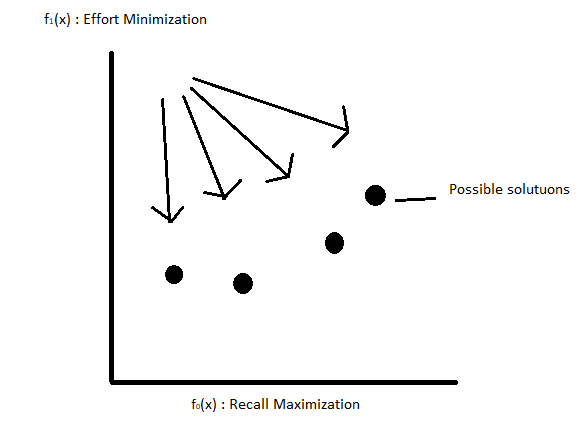
\includegraphics[width=11cm]{figures/MOGA.png}
\caption{MOGA algorithm using various search directions. Image reproduced from \cite{489161}}
\end{figure}


\subsection{Existing Stopping Methods} \label{methods}

As discussed in \ref{stops}, existing methods for finding stopping points in ranked documents have been proposed.

\subsubsection{Target} \label{target}

The target method is an approach that can guarantee a certain a certain level of reliability \ref{evalsstops}. It was first proposed by Cormack and Grossman \cite{Cormack2016}. This method randomly samples returned documents until a target number $T$ of relevant document are found.

The target $T$ denotes how many documents we should randomly select from our initial query. A larger value of $T$ will increase the effort required as we are more likely to select a document towards the end of the query set. Documents are looked at until the target point $T$ has been reached.

We first compute a random target set of relevant documents. We then calculate the last document in the target set and mark that as our target point:

\begin{equation}
	  \underset{last}{d} = \underset{d \in{T}}{argmax relrank(d)}
\end{equation}

It must hold that $d$ is in the target set. $relrank$ determines whether or not a document is relevant.

\begin{figure}[H]
\center
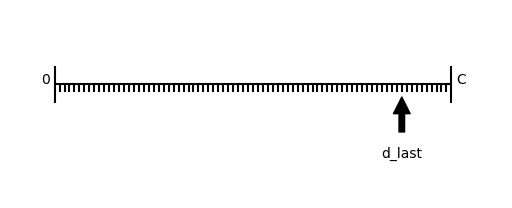
\includegraphics[width=9cm]{figures/target_method.png}
\caption{Visualisation of target method last relevant document selection. $C$ is number of documents in collection.}
\end{figure}

Increasing our target set size is likely to increase the probability the last document being towards the end of the document collection.

We can calculate the recall of the point by looking at the relevance rank of the last document:

\begin{equation}
	  recall = \frac{relrank(\underset{last}{d})}{R}
\end{equation}

Where $R$ is the number of relevant documents.


For our method to be deemed reliable we must achieve 70\% recall with a 95\% average over all topics.

\begin{equation}
	  P(\frac{relrank(\underset{last}{d})}{R} \geqslant 0.7) \geqslant 0.95
\end{equation}


Assuming we have a large number of relevant documents $R$ we need to determine cut-off $c$

\begin{equation}
	  P( \frac{R - relrank(\underset{last}{d})}{R} > c) = 0.05
\end{equation}

This can be further simplified to:

\begin{equation}
	  P(R - relrank(\underset{last}{d}) > cR) = 0.05
\end{equation}

Which translates to the probability of the remaining relevant documents being higher than the cut-off point should be 0.05.

For this to hold, $cR$ documents must be absent from $T$. This occurs with the probability:


\begin{equation}
	  \left(1 - \frac{10}{R}\right)^{cR} = 0.05
\end{equation}

Which can become:

\begin{equation}
	  c = \frac{log(0.05)}{R log(1 - \frac{10}{R})}
\end{equation}


In cases where $R$ has more than 10 relevant documents it follows:


\begin{equation}
	  c < \lim_{R \to \infty} \frac{log(0.05)}{R log (1 - \frac{10}{R})} = 0.299573 < 0.3
\end{equation}

Finally we have:

\begin{equation}
	 R \leq 10 \cup P(\frac{relrank(\underset{last}{d})}{R} \geq 0.7) 	\geq 0.95
\end{equation}

Overall, while the target method is shown to acquire 95\% reliability, the effort needed is often significantly high, often requiring us to look at huge volume of documents.



\subsubsection{Knee Method} \label{knee}

A different stopping kethod proposed by \cite{Satopa11} is known as the knee method. This approach uses a curve to generate a 'knee', which is then used for predicting a stopping point. This approach is likely to be highly dependant on the quality of the initial rankings. This is because we need a curve that reaches a peak quickly, before flattening out.

We use a vertical line panning the length of the ranking set and use it to calculate the distance from the ranking at each point. The point with the maximum distance is chosen as a suitable stopping point.

\begin{figure}[H]
\center
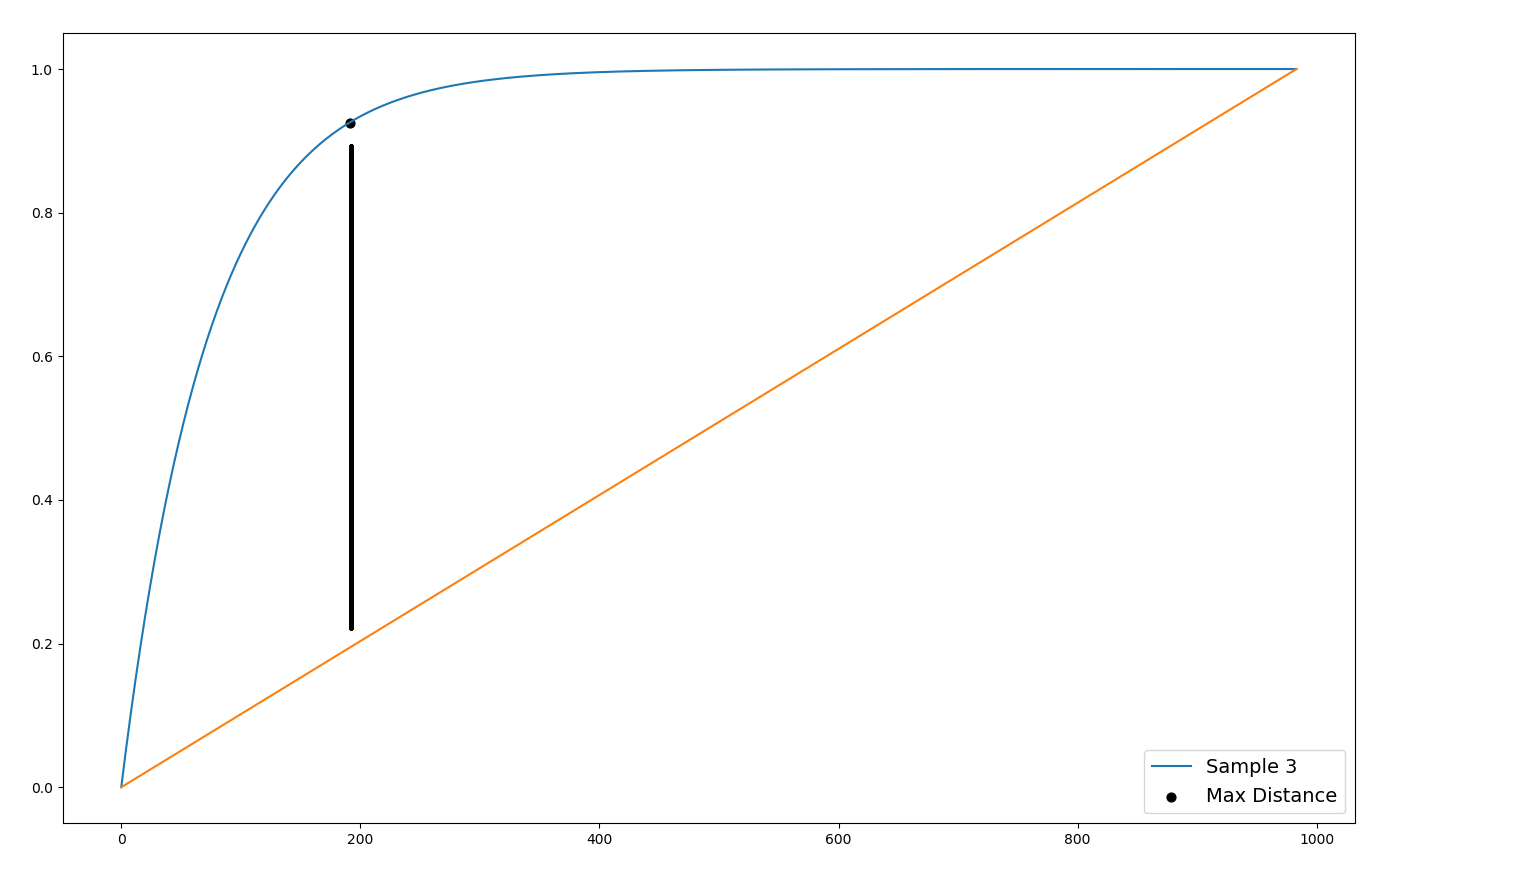
\includegraphics[width=13cm]{figures/knee.png}
\caption{Example of using knee method to find a stopping point. Image inspired from \cite{Satopa11}}
\end{figure}

We can see in the above example the method has predicted we look at around 200 of the 1000 documents to achieve a suitable stopping point.

This method also imposes an additional constraint for rankings of a large volume. 

It was found that the knee method is a better approach for finding a stopping point than the Target method \cite{Cormack2016}. The recall was always found to be better and the reliability was found to be the same or higher for 6 out 8 test collections.



\section{Summary} \label{sumlit}

We first examined the steps of a systematic review \ref{stepssr} and looked at potential areas to introduce NLP techniques. We broke down the stages of a systematic review such that we can examine what techniques we could apply at each stage. 

We then began to examine stopping criteria \ref{stops}. We looked at the intuition behind looking for stopping points in ranked sets of documents. We defined our stopping problem as a multi-objective optimization problem \ref{stoppingProblem}. We looked into two existing approaches, the target method and the knee method.


